\documentclass[10pt,twocolumn,letterpaper]{article}

\usepackage{cvpr}
\usepackage{times}
\usepackage{epsfig}
\usepackage{graphicx}
\usepackage{amsmath}
\usepackage{amssymb}
\usepackage{subfigure}

% Include other packages here, before hyperref.

% If you comment hyperref and then uncomment it, you should delete
% egpaper.aux before re-running latex.  (Or just hit 'q' on the first latex
% run, let it finish, and you should be clear).
\usepackage[breaklinks=true,bookmarks=false]{hyperref}
\cvprfinalcopy % *** Uncomment this line for the final submission

\def\cvprPaperID{****} % *** Enter the CVPR Paper ID here
\def\httilde{\mbox{\tt\raisebox{-.5ex}{\symbol{126}}}}

% Pages are numbered in submission mode, and unnumbered in camera-ready
%\ifcvprfinal\pagestyle{empty}\fi
\setcounter{page}{1}
\begin{document}

%%%%%%%%% TITLE
\title{toon2real: Translating Cartoon Images to Realistic Images}

\author{Labiba Kanij Rupty \\ {\tt\small labknr98@gmail.com} 
\and Mohammad Imrul Jubair \\ {\tt\small mohammadimrul.jubair@ucalgary.ca}
\and K M Arefeen Sultan \\ {\tt\small krsultan069@gmail.com}
\and Sayed Hossain Khan \\ {\tt\small sayedhossainkhan36@gmail.com}
\and MD. Nahidul Islam \\ {\tt\small nahidul19967@gmail.com}
\\
\and Department of CSE, Ahsanullah University of Science \& Technology, Bangladesh.
} 

\maketitle
%\thispagestyle{empty}

%%%%%%%%% ABSTRACT
\begin{abstract}
In this paper, we encounter the challenge of translating cartoon images to realistic images. As the Generative Adversarial Networks have tremendous successes in image-to-image translation, its variants drew our attention to perform the task. We prepared unpaired datasets for both cartoon and realistic domains, and we discerned that CycleGAN is suitable to reach our goal---as its Cycle-Consistency loss function is fit for working with unpaired datasets.
We applied this model and the results exhibit that our approach produces satisfactory realistic images from cartoon images.

\end{abstract}

%%%%%%%%% BODY TEXT
\section{Introduction}
%Since the revolution of digitization,
Movies 
%have served 
serve
%the humanity 
as one of the most popular sources of entertainment for human beings. Cartoons, undeniably, held a large part of entertainment industry in this modern day world.
While watching them,
%didn't this ever come to one's mind
%Naturally, 
a curiosity might be prompted in our mind:
\textit{How enchanting it would be to see our favourite cartoons become realistic? What if the adventure of Chihiro from \textit{`Sprited Away (2001)'} is rendered in a real-life setup?
%that we see in live action movies?
Or the journey of Carl from \textit{`Up (2009)'}?}

We reckon the above fantasy crosses most of the cartoon lovers' minds once in a while; however, making this happen in reality
%has never been 
is not
an easy task.
%From \cite{aramide-tinubu2018Nov, Bacon2019Feb}, we get to know that, 
For instance,
an upcoming movie \textit{`The Lion King (2019)'}---remake of one of the most popular animated movies \textit{`The Lion King (1994)'}---costs four times
%of 
the
%cost of its 
original one \cite{aramide-tinubu2018Nov, Bacon2019Feb}. The reason
%behind this 
is that the new movie is a live-action version of the animated one based on Computer-Generated Imagery (CGI) which is a costly task to perform \cite{BibEntry2015Jun}. Moreover, the time and the labour required to generate an image are also high.

In this paper, we consider the above subject as our research problem and we attempt to
%we 
%contribute
%to this problem domain 
%by 
%proposing
%we 
propose 
a
%much less time consuming and a more cost-saving
time \& cost effective
solution. We aim to input a cartoon image and to produce its realistic version automatically. Hence, we present a technique called \textbf{\textit{``toon2real''}}---a Generative Adversarial Networks (GANs)~\cite{goodfellow2014generative} based approach---that translates cartoons to realistic images.
%Although 
There has been some tremendous researches on image-to-image translation using GANs such as \cite{yu2018singlegan, CycleGAN2017, liu2017unsupervised, isola2017image, karras2018style}; however, to our knowledge there hasn't been any research on generating realistic images from cartoon images yet. The closest research on translating cartoon images to realistic images has been touched by Li \etal \cite{li2018twin} which only covers the face generation part of the task. Besides, Tomei \etal translates art images to realistic domain in their work \cite{tomei2018art2real}, where each object of an image from the cartoon is mapped with the same objects from images of realistic domain.
Moreover, the CartoonGAN \cite{chen2018cartoongan}---a motivation behind our work---converts real image to cartoon; performing contrariwise is not a solution to our problem as the detail preservation from real to cartoon is not similar for vice versa.
Hence, translating cartoons to realistic images is much harder because the cartoon images are smoothed out and their details are very trivial while compared to realistic images.

In this paper, we apply a technique which is based on CycleGAN \cite{CycleGAN2017} to achieve desired goal. We demonstrate our results and, in addition, we compare it with the UNIT method used by Liu \etal \cite{liu2017unsupervised}.
%and enhanced version of CycleGAN\cite{CycleGAN2017} where 
%Moreover, we added an additional loss function based on WGAN-GP \cite{gulrajani2017improved} and examine its performance.
%-------------------------------------------------------------------------
\section{Formulation}
%Our main objective is to translate images of \textit{cartoon} domain to \textit{realistic} domain by learning the mapping of a \textit{cartoon} domain $C$ to the \textit{realistic} domain $R$.
Our main objective is to translate images of \textit{cartoon} domain ($C$) to \textit{realistic} domain ($R$) by learning the mapping of $C$ to $R$. 
To satisfy this requirement, we adopt the {CycleGAN}~\cite{CycleGAN2017} method to train our models. Our overall approach is discussed below.
%along with the process of dataset preparation.

\subsection{Data Collection}
Due to the lack of paired datasets between \textit{realistic} and \textit{cartoon} domain, we took an approach to collect unpaired datasets for both domains. Initially, for \textit{realistic} domain, we scraped scenery images from \textit{Flickr} and many other sources which were tagged as \textit{scenery, sunrise, sunset, sea, sky} \& \textit{beach} and collected around $7K$ samples.
Besides, for \textit{cartoon} domain, we extracted images from various Japanese anime movies. We excluded the frames which are darker to see, and the first and last few frames---as the introductory and credits part tend to be textual in a movie.
After hand-picking the appropriate images, in order to approximate with the size of the \textit{realistic} domain, we collected images from more than $15$ cartoon movies and clips. For both the domain, images were of $128\times 128$ dimension.

\subsection{Model Development}

To train our datasets the CycleGAN model is exploited. In this subsection, we discuss GANs very briefly followed by two key concepts of CycleGAN: the {Cycle-Consistency loss} and the PatchGAN.

\parindent 5ex \textbf{Generative Adversarial Networks (GANs):} $Two$ networks will simultaneously learn the probability distribution of two domains---in our case, they are the cartoon domain $C$ and the realistic domain $R$---to defeat each other. The first network is a generator, $G_r: C\rightarrow R$ which learns the mapping between the distribution of domain $C$ and $R$ and will generate fake images $r_{fake}$, matched to $R$, whereas the second network,  Discriminator $D_r$ will learn the probability distribution of $R$ and try to differentiate between the generated images, $r_{fake}$ and the images $r$ from $R$. GANs generate images by minimizing the differences between the original content and the newly generated distribution. The measurement of the difference is named as \textit{adversarial loss}. Goodfellow \etal \cite{goodfellow2014generative} proposed a binary cross-entropy loss function, however, we used \textit{least squares loss} function as our \textit{adversarial loss} as it shows more stability according to Mao \etal \cite{DBLP:conf/iccv/MaoLXLWS17}.

\parindent 5ex \textbf{Cycle-Consistency Loss:}
%Due to the fact that
As
we
%are using 
use
unpaired datasets, exclusively applying adversarial loss produces images
%which 
failing to match with the input data. As a result, while generating a realistic image from cartoon image, because of the void mapping, the model tends to depict random realistic images without considering the distribution of cartoon image. However, in case of \textit{Cycle-Consistency Loss} function \cite{CycleGAN2017}, the model learns from the most closely matched distribution of the domain. The motive of this function is that, an image generated from an input can be reconstructed back to the input again such that $x = F(G(x))$, where $F$ and $G$ are generators and $x$ is the input, and thus it is able to map an image of target domain which is as close as possible to the image of input domain.
In Equation~\ref{cyc}, the loss function is showed where, $m$ is the total number of images for each domain, and $c$ \& $r$ are the samples from the domain $C$ and $R$ respectively.
\begin{equation}
\label{cyc}
\mathcal{L}_{cyc} = \frac{1}{m} \sum^m_{i=1}(F_r(G_r(c)) - c) + \frac{1}{m} \sum^m_{i=1}(G_r(G_c(r)) - r)
\end{equation} 


\parindent 5ex \textbf{PatchGAN:}
As discriminators, PatchGAN model is used which was first proposed by Isola \etal
\cite{isola2017image}.
It has a 
%Another 
beneficial feature 
%is that due to
of
working on $N\times N$ patches; it takes fewer parameters and thus decreases the computational cost. The method works best for extracting the high-frequency details of the distribution.

%-------------------------------------------------------------------------

\section{Results}
We present our results followed by the comparison with UNIT~\cite{liu2017unsupervised} and our failed cases in Figure~\ref{fig:results},~\ref{fig:comparison} and~\ref{fig:limitation} respectively. Our approach produces great results which is clear in Figure~\ref{fig:results}. Also, we choose the \textit{Fr\'echet Inception Distance (FID)} \cite{heusel2017gans} for quantitative evaluation. It shows more consistency with the human evaluation as the measurement is based on the difference between the generated and the actual dataset. We measured our output and the output of UNIT in terms of FID score where ours show the least FID score, $40.38$ compared to UNIT's, which is $59.78$. Here, the lower the FID score, the better the result is.


\section{Discussions}
%In this section, we will, at first, discuss the limitations of our approach and what we are planning to do in future. Later, we will talk about the implications of this study.
In this paper, we ventured to contribute to the entertainment sector by presenting cartoons to realistic image translation. We applied CycleGAN approach which nicely adapts our unpaired datasets of cartoon and realistic domain. The experimental results show that our method performs adequately to produce desired outcomes. However, as an evolving research, it has certain limitations and we scheme to overcome those, which are shortly discussed below.

%\parindent 5ex \textbf{Limitations \& Future Plans:}
Despite producing the lowest FID score, it is still high which implies that there is still chance to improve. Besides, our technique currently works for scenery based images and fails to generate geometric structure from any cartoon image, e.g. human figure. From Figure~\ref{fig:limitation}, we can see that the method fails to translate a human figure as it is unaware of the semantic representation.
%Geometric structure.

To improve the FID score, we have plans to train the datasets semantically, which is instead of training the entire images, we will train their segmented versions. Hence, the objects, e.g. trees, from cartoon domain will be segmented and mapped to the similar objects (trees) in the real domain \cite{mo2018instagan, tomei2018art2real}.

%Besides, right now, we need almost $5$ days to train our model on \texttt{NVIDIA GEFORCE GTX 1060}. Our plan is to minimize the time.

%-------------------------------------------------------------------------
%-------------------------------------------------------------------------


\begin{figure*}[!htb]
\centering     %%% not \center
\subfigure
{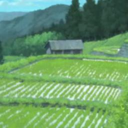
\includegraphics[width=30mm]{best_ones/4999_real_A.png}}
\subfigure
{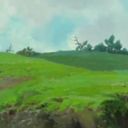
\includegraphics[width=30mm]{best_ones/5407_real_A.png}}
\subfigure
{
\includegraphics[width=30mm]{best_ones/5130_real_A.png}}
\subfigure
{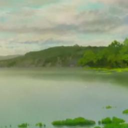
\includegraphics[width=30mm]{best_ones/5468_real_A.png}}
\subfigure
{\label{fig:a}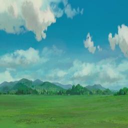
\includegraphics[width=30mm]{best_ones/616_real_A.png}}

\subfigure
{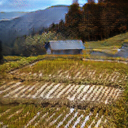
\includegraphics[width=30mm]{best_ones/4999_fake_B.png}}
\subfigure
{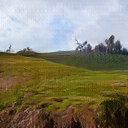
\includegraphics[width=30mm]{best_ones/5407_fake_B.png}}
\subfigure
{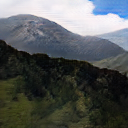
\includegraphics[width=30mm]{best_ones/5130_fake_B.png}}
\subfigure
{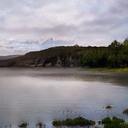
\includegraphics[width=30mm]{best_ones/5468_fake_B.png}}
\subfigure
{\label{fig:res_b}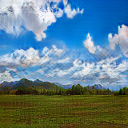
\includegraphics[width=30mm]{best_ones/616_fake_B.png}}

\caption{\textit{\textbf{Our results:}} The \textit{first row} represents the input images from cartoon domain and \textit{second row} shows the corresponding outcomes. It can be observed intuitively that the results are vivid and realistic.}
\label{fig:results}
\end{figure*}

\begin{figure}[!htb]
\centering     %%% not \center
\subfigure[Input]
{\label{fig:com_in}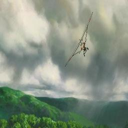
\includegraphics[width=27mm]{Comparisons/52_real_A.png}}
\subfigure [CycleGAN]
{\label{fig:com_a}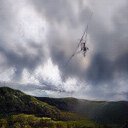
\includegraphics[width=27mm]{Comparisons/cycle_52.png}}
\subfigure [UNIT]
{\label{fig:com_b}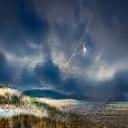
\includegraphics[width=27mm]{Comparisons/UNIT_52.jpg}}

\caption{\textit{\textbf{Ours vs. UNIT:}}
%The input of these two figures are referenced in Figure~\ref{fig:res_b}. 
(b) shows the output of our proposed method which perfectly keeps the content of the input (a) and is visually sensible. It is far more realistic compared to the result of applying UNIT \cite{liu2017unsupervised} (c) that fails to keep the content of the input.}
\label{fig:comparison}
\end{figure}

\begin{figure}[!htb]
\centering     %%% not \center
\subfigure [Input]
{\label{fig:lim_a}
\includegraphics[width=24mm]{limitations/435_real_A.png}}
\subfigure [Output]
{\label{fig:lim_b}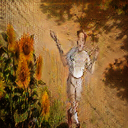
\includegraphics[width=24mm]{limitations/435_fake_B.png}}

\caption{\textit{\textbf{Our limitations:}} An unsuccessful case (b) of our method where it fails to translate the human figure for the input image (a).}
\label{fig:limitation}
\end{figure}
%------------------------------------------------------------------------

{\small
\bibliographystyle{ieee}
\bibliography{egbib}
}

\end{document}
